Das folgende Kapital beschreibt die statische Grunstruktur des Systems sowie
deren Funktionalität.
{
\bf
Es ist zu beachten, dass sämtliche Diagramme und Beschreibungen in diesem
Abschnitt nur zur Verdeutlichung der Systemarchitektur dienen und noch
keinen Anspruch auf Vollständigkeit erheben. Für alle Arbeiten an einem Modul
ist unbedingt dessen aktuellste Dokumentation zu verwenden.
}

\begin{figure}[H]
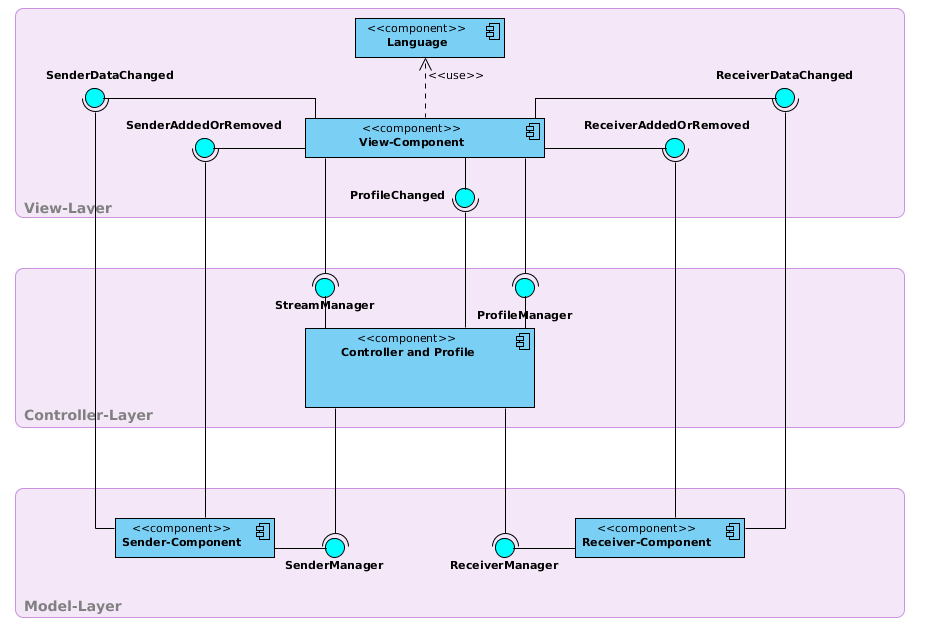
\includegraphics[width=15cm]{images/Overview.png}
\centering
\caption{Komponentendiagramm: Gesamtsystem}
\label{uml_controller}
\end{figure}

Das Gesamtsystem ist zeitgemäß nach dem Model-View-Controller-Entwursmuster
aufgebaut. Dabei werden Programmlogik (Model) und Darstellung (View) voneinander
entkoppelt und kommunizieren über eine Steuerschicht (Controller) miteinander.
Auf diese Weise wird es möglich, die eigentliche Programmlogik direkt für
verschiedene Darstellungsformen zu verwenden. Im Falle des Multicast-Test-Tools
handelt es sich dabei um die graphische Oberfläche (GUI) sowie die
Kommandozeilen-Invokation mit Logger (CLI/Logger). Die graphische Oberfläche ist
weiterhin eingeteilt in einen Darstellungs- und einen Logik-Teil. Die
Anforderung Konfigurationsdateien erstellen und laden zu können, wurde mit den
Profilen des Controllers verwirklicht. Weiterhin wurde das System nach
folgenden Prinzipien modelliert:
\begin{itemize}
  \item Einfache Erweiterbarkeit durch Nutzung des Beobachter-Muster
  (Observer-Pattern) an angemessenen Stellen.
  \item Auslagerung von Logik in eine eigene Klasse nach Strategie-Muster
  (Strategy-Pattern) um Programmfehler durch erwartete, häufige
  Änderungsanfordungen zu vermeiden. Beim MC-Test-Tool wurde das Paketformat auf
  diese Weise in das Paket-Komponente (Packet) ausgelagert.
  \item Geringe Kopplung durch Abstraktion und Schnittstellen-Nutzung.
\end{itemize}

\section{Controller/Profile}
\label{sec:4:steuer}
\begin{figure}[H]
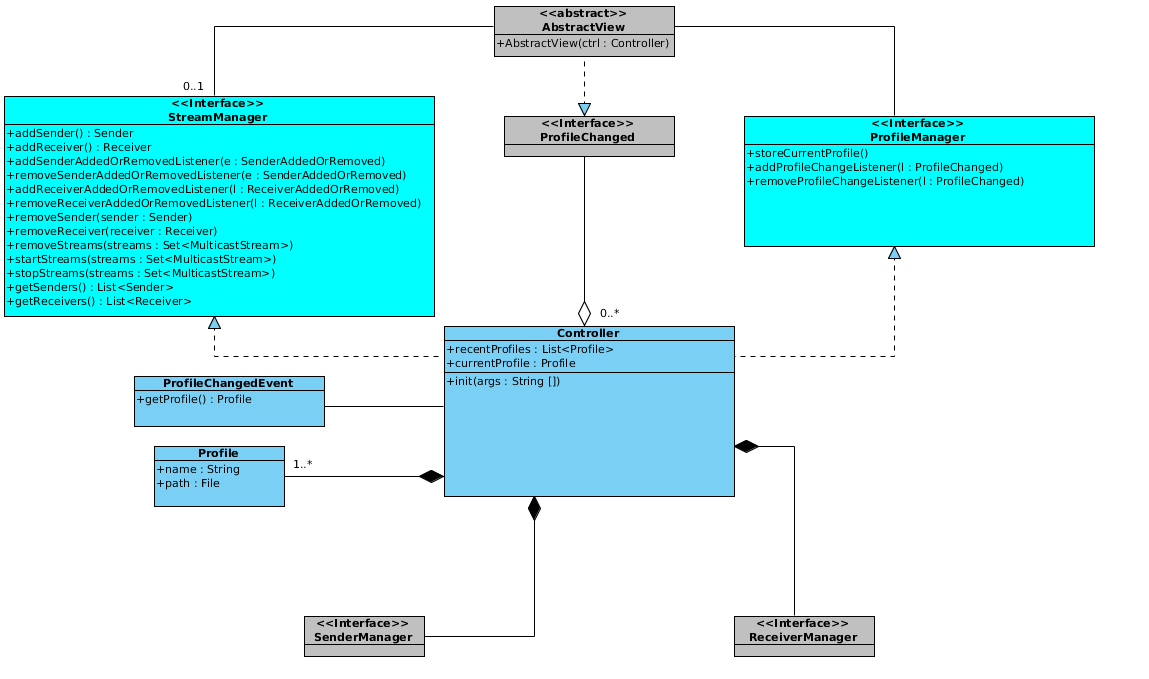
\includegraphics[width=15cm]{images/Controller.png}
\centering
\caption{Klassendiagramm: Controller/Profile - Komponente}
\label{uml_controller}
\end{figure}

\paragraph{Zweck}
Die Controller-Komponente ist der Einstiegspunkt des Systems. Sie erhält beim
Programmstart vom Nutzer alle nötigen Informationen zu dessen Anwendungsabsicht
und entscheidet welche Komponenten auf welche Weise initiliasiert werden müssen.
Danach erstellt sie nach diesen Anforderungen die benötigten Model- und
Viewkomponenten und dient als Kommunikationszentrale zwischen diesen und der
Konfiguration. Die 
\textbf{Profile}-Komponente repräsentiert den Namen und Dateipfad
einer XML-Datei, welche eine mögliche Konfiguration des Programms enthält.
Die Konfigurationsdateien stellen XML-Serialisierungen des momentanen
Controller-Zustands sowie der Ausprägung des Sender- und Receiver-Pools dar.
\paragraph{Erfüllte Anforderungen}
/VA0600/, /QZ10/
\paragraph{Variablität}
volatil - gefestigt
\paragraph{Qualitätsmerkmale}
Änderbarkeit, Anpassbarkeit
\paragraph{Offene Punkte}

\section{Sende- und Empfangsmodul}
\label{sec:4:send}
\begin{figure}[H]
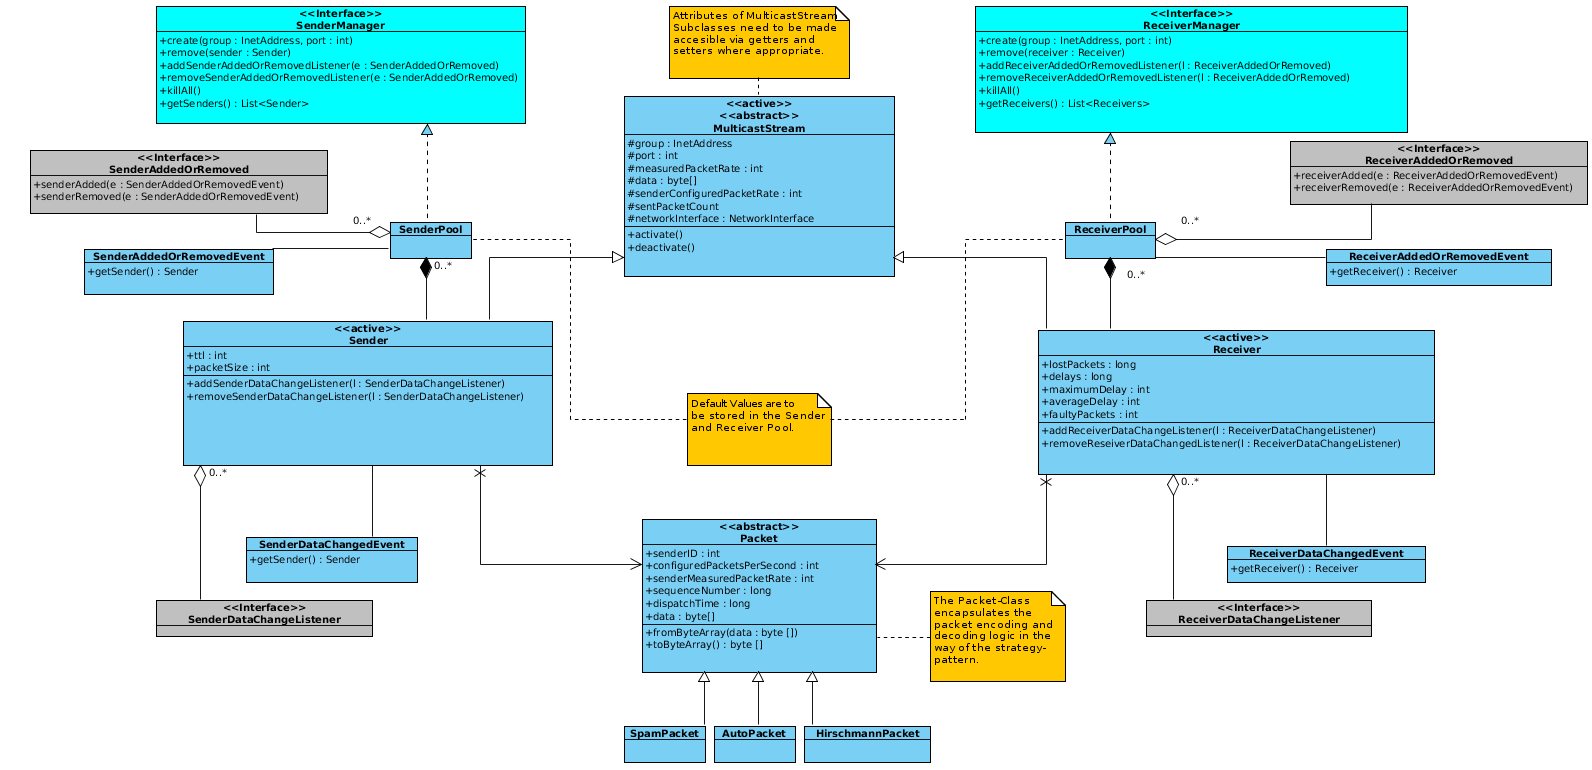
\includegraphics[width=18cm]{images/Model.png}
\centering
\caption{Klassendiagramm: Sende-/Empfangskomponente}
\label{uml_controller}
\end{figure}

\paragraph{Zweck}
Die Sende- und Empfangskomponente des Systems stellt gleichzeitig dessen Kern
dar. Sie besteht aus einer aktiven \textbf{Sender}- und \textbf{Receiver}-Klasse,
die auf Intanzebene jeweils einen sendenden oder empfangenden Datenstrom
repräsentiert. Die Instanzen dieser Klassen arbeiten parallel und autonom in der
Model-Schicht des Systems, erheben alle definierten Daten und informieren alle
Komponenten die die Multicast-Datenstrom Informationen benötigen über die
Schnittstellen \textbf{ReceiverDataChangeListener} und
\textbf{SenderDataChangeListener}. Außerdem existiert jeweils eine
\textbf{SenderPool} und eine \textbf{ReceiverPool} Klasse, die als Container für alle konfigurierten
Datenstrom-Instanzen fungiert und diese verwaltet. Bei Änderungen der
Datenströme, werden interessierte Komponenten über die \textbf{SenderAddedOrRemoved}
bzw \textbf{ReceiverAddedOrRemoved} Schnittstelle benachrichgt.
\paragraph{Erfüllte Andorderungen}
VA0100, VA0200, VA0300, VA0500, VA0800, VA1000, VA1300, OA0100, OA0400
\paragraph{Variablität} gefestigt
\paragraph{Qualitätsmerkmale}
QZ10, QZ30, QZ50, QE10, QP10, QP20, QP40
\paragraph{Offene Punkte}
OP0300 - Verzögerungen?

\section{Paketkomponente}
\label{sec:4:empf}
\begin{figure}[H]
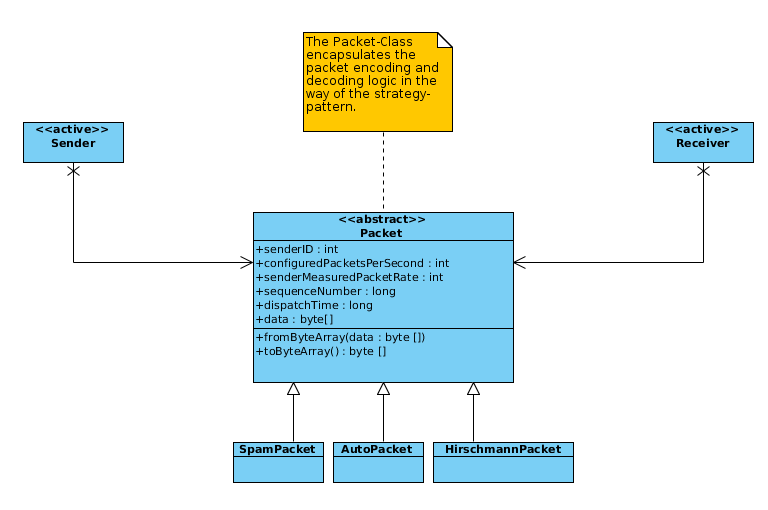
\includegraphics[width=15cm]{images/Package.png}
\centering
\caption{Klassendiagramm: Paketkomponente}
\label{uml_controller}
\end{figure}

\paragraph{Zweck}
Dieses Modul stellt die für die Erkennung und Erstellung von Multicast Paketen 
erforderlichen Funktionalitäten zur Verfügung. Hierbei werden Details über die 
tatsächliche Implementierung des Bitstreams eines Paketes hinter einem 
einheitlichen Interface verbogen. Dies wird unter anderem dadurch erreicht, dass
das Format eines ankommenden Pakets automatisch erkannt wird.
\paragraph{Erfüllte Anforderungen}
/VA0400/, /OA0400/, /QF20/, /QF40/, /QZ20/, /QZ30/, /QZ40/ 
\paragraph{Variablität}
volatil - gefestigt
\paragraph{Qualitätsmerkmale}
Änderbarkeit, Anpassbarkeit, Robustheit
\paragraph{Offene Punkte}

\paragraph{Protokoll Spezifikation}

Um die Testbarkeit eines Multicast Netzwerkes zu ermöglichen, muss das Tool notwendigerweise
Datenpakete via Multicast versenden können. Die versendeten Pakete müssen Informationen über den
Zustand der Applikation zum Zeitpunkt des Versands beinhalten, um so beim Empfänger
Statistiken über die Übertragung erstellen zu können. Um die nötigen Informationen
zu strukturieren ist ein Datenformat von Nöten. Die Struktur sollte einfach
Erweiterbar und trotzdem simpel gehalten sein um das Dekodieren der Pakete 
effizient zu gestalten. Das TLV Protokoll erfüllt all diese Anforderungen.
TLV steht für Type-Length-Value-Format und wird in vielen vorhandenen 
Netzwerkprotokollen, wie zum Beispiel COPS, IS-IS, LLDP und RADIUS genutzt,
wobei es sich dort als erweiterbar und robust bewährt hat.
Bei diesem Protokoll wird jedes Attribut eines Paketes durch folgendes Tripel übermittelt:

\begin{itemize}
 \item[-] Type: bestimmt den Typ des Attributes, in unserem Fall ein unsinged 
                16bit Integer.
 \item[-] Length: bestimmt die Länge des Attribut Wertes und ist 
                  in unserem Fall ein unsigned 32bit Integer.
 \item[-] Value: enthält den eigentlichen Wert des Attributes.
\end{itemize}

Durch die einheitliche Struktur des Protokolls ist es sehr einfach Sequenzen von
TLV Tripel mit einer einheitlichen Funktion zu durchsuchen.
Hierbei werden Tripel mit einem unbekannten Typen ignoriert, was zu einer 
einfachen Erweiterbarkeit führt. Die Anzahl der Tripel im Paket muss nicht 
angegeben werden, da die Länge des Paketes schon im UDP Header enthalten ist.
Zudem kümmert sich UDP auch um die Integrität der Daten, ein extra CRC Hash oder
Paritybits müssen also nicht mit übertragen werden. Alle Datenfelder werden
im Big Endian Format representiert.
\\ \\
Um das hier spezifizierte Protokoll vom Hirschmann-Protokoll und anderen
Protokollen zu unterscheiden, ist ein Header vor den TLV Attributen wichtig. Daher muss vor dem ersten TLV Trippel 
folgendes Hexadezimales Bytemuster stehen.
\\ \\
05 39 00 00 00 00
\\ \\
Diesen Header kann man auch als TLV Trippel mit dem Typ 1337, der Datenlänge
0 und keinen Nutzdaten auffassen. Dieser Umstand vereinfacht potentiell das parsen des Protokolls.
\\ \\
\textbf{Das Protokoll kann wie folgt als DD dargestellt werden:} \\ \\
Paket = Header + {TLV} \\
Header = 0x053900000000 \\
TLV = Type + Length + Value  \\
Type = 0..65535  \\
Length = 0..4294967295 \\
Value = Datenstrom der zuvor genannten Länge. \\
\\ 
\begin{table}[htdp]
\centering
\caption{Im Protokoll verwendete Attribute}
\label{tab:prot}
\begin{tabular}{|l|l|p{9.5cm}|}
\hline
\textbf{Beschreibung} & \textbf{Typ} & \textbf{Attribut Wert} \\
\hline
Sender ID & 1 & Signed 32bit Integer Sender ID.\\
\hline
Eingestellte Paketsenderate & 2 & Pakete pro Sekunde als unsigned 32 bit Integer. \\
\hline
Ermittelte Paketsenderate & 3 & Pakete pro Sekunde als unsigned 32 bit Integer. \\
\hline
Sequenznumber & 4 & Signed 32bit Integer Sequenznumber. \\
\hline
Absendezeit & 5 & Nanosekunden seit dem 1. Januar 1970 00:00 Uhr UTC (vergleiche Unixzeit) als signed 64 bit Integer. \\
\hline
Daten & 6 & Datenstream variabler Länge. \\
\hline
Padding & 7 & Feld zum Auffüllen des Pakets auf eine bestimmte Länge. \\
\hline
\end{tabular}
\end{table}


\section{Language}
\label{sec:4:pakdef}
% uml ausschnitt
\begin{figure}[H]
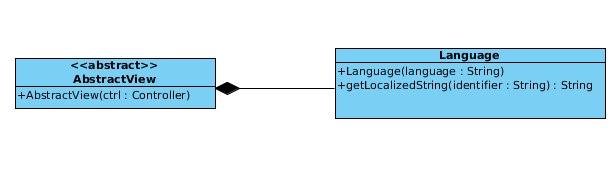
\includegraphics[width=15cm]{images/Language.png}
\centering
\caption{Klassendiagramm: Internationalisierungs-Komponente}
\label{uml_controller}
\end{figure}

\paragraph{Zweck}
In diesem Modul werden alle Internationalisierungsdetails hinter einem sehr einfachen Interface verborgen.
Die Komponente kümmert sich um das laden der Sprachdateien und übersetzt übergebene Template Strings 
in die gewählt Sprache und kümmert sich zudem um die Ersetzung von Platzhaltern in den Strings und
die übersetzung von Exceptions.
\paragraph{Erfüllte Anforderungen}
/QU70/
\paragraph{Variablität}
volatil - gefestigt
\paragraph{Qualitätsmerkmale}
Änderbarkeit, Anpassbarkeit, Simplizität
\paragraph{Offene Punkte}

\section{GUI-Design}
\label{sec:4:konf}
\begin{figure}[H]
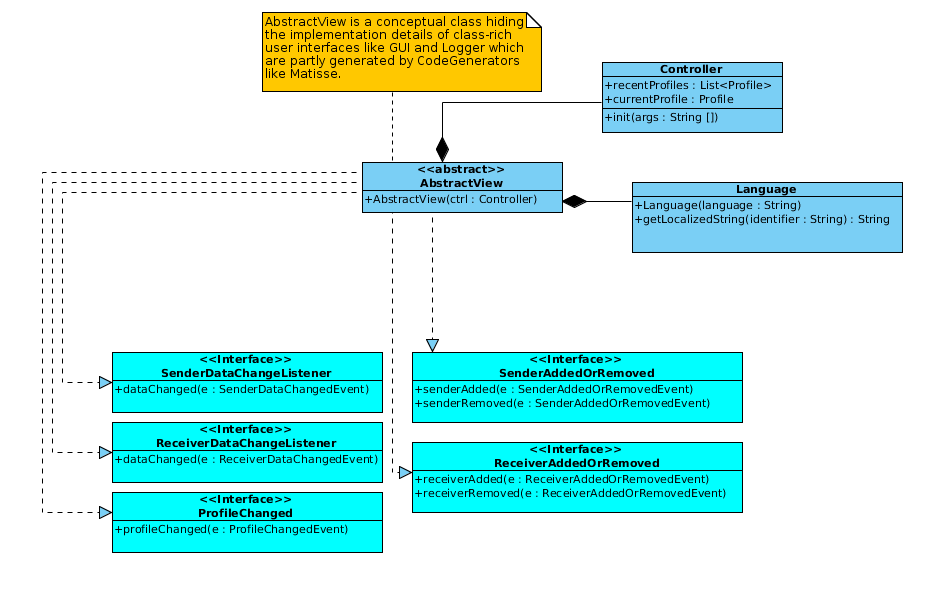
\includegraphics[width=15cm]{images/View.png}
\centering
\caption{Klassendiagramm: View-Komponente}
\label{uml_controller}
\end{figure}

\paragraph{Zweck}
In diesem Modul wird vorallem die konkrete Implementierung der GUI abstrahiert. 
Hierzu gehören beispielsweise die Position von Bedienelementen oder
die Art der Bereitstellung von Benutzeraktionen (Shortcuts, Menüs, Button). 
Dieses Modul hat eine relativ starke Bindung zur Logik der GUI. Ein Model für
eine mögliche Implementierung der GUI ist im Anhang vorhanden. Zu beachten ist
dabei, dass die grafische Darstellung der Datenstromstatistiken nur eine
optionale Anforderung ist.
\paragraph{Erfüllte Anforderungen}
/UC10/, /VA0700/, /VA0800/, /VA1000/, /VA1100/, /VA1200/, /OA0300/, /QF10/, /QU10/, /QU20/, /QU30/, /QU40/, /QU50/, /QU60/
\paragraph{Variablität}
gefestigt
\paragraph{Qualitätsmerkmale}
Änderbarkeit, Anpassbarkeit, guter Look and Feel, Simplizität
\paragraph{Offene Punkte}

\section{GUI-Logik}
\label{sec:4:konf}

\paragraph{Zweck}
Dieses Modul kapselt die Logik der GUI. Hierzu gehört zum Beispiel die 
Umsetzung von Models, welche den einzelnen Swing Komponenten ihre Daten liefern.
Zudem werden hier Konfigurationen gespeichert und geladen.
Dieses Modul hat eine relativ starke Bindung zum Design der GUI. 

\paragraph{Erfüllte Anforderungen}
/UC10/, /VA0700/, /VA0800/, /VA1000/, /VA1100/, /VA1200/, /OA0300/, /QF10/, /QU10/, /QU20/, /QU30/, /QU40/, /QU50/, /QU60/

\paragraph{Variablität}
gefestigt
\paragraph{Qualitätsmerkmale}
Änderbarkeit, Anpassbarkeit
\paragraph{Offene Punkte}

\section{CLI/Logger}
\label{sec:4:konf}

\paragraph{Zweck}
Diese Komponente beinhaltet die Funktionalität, das Programm auf
Kommandozeilenebene zu steuern (im genaueren den Start des Programms mit einer
existieren Konfigurationsdatei und der Definition ob nur die Sendenden,
Empfangenden oder alle Datenströme geladen werden sollen). Dies umfasst die
Definition und Dokumentation des Kommandozeilenaufrufs sowie die Implemtierung
der \textbf{ArgumentParser}-Klasse, die eine Reihe von Kommandozeilenargumenten
in dieser Hinsicht interpretiert. Die Logger-Funktionaltität muss als
View-Komponente implementiert werden. Sie erhält damit von den Datenströmen
regelmäßig statistische Informationen und muss diese in einer Log-Datei
persistieren.
\paragraph{Erfüllte Anforderungen}
/UC20/, /VA0900/, /QF30/
\paragraph{Variablität}
volatil
\paragraph{Qualitätsmerkmale}
Änderbarkeit
\paragraph{Offene Punkte}
Log-Format als Fließtext, XML oder konfigurierbar?\\
Detailierung\\

\section{Installer}
\label{sec:4:konf}
\paragraph{Zweck}
Einfache Installation unter Windows und Linux Debian.
\paragraph{Erfüllte Anforderungen}
/QP30/
\paragraph{Variablität}
volatil
\paragraph{Qualitätsmerkmale}
Einfache Bedienbarkeit
\paragraph{Offene Punkte}
Je nachdem Java WebStart?
